\chapter{Introduction}
\vskip 0.1in
\indent
\indent

This project has been developed as part of the BSC(Honours) in Science in Computing in Software development course for the module minor project and dissertation on the last year of a fourth-year course. The module corresponds to 15 credits out of 60 in the year. 

Two students have developed the project, which has been divided into two parts: front-end and back-end, Elena was is developed the front-end and Jose the back-end.

We have developed a microservice application using go as a principal back end programming language, with a react native client and a REST-API(Figure \ref{application:uml}).
\begin{figure}
	\begin{center}
		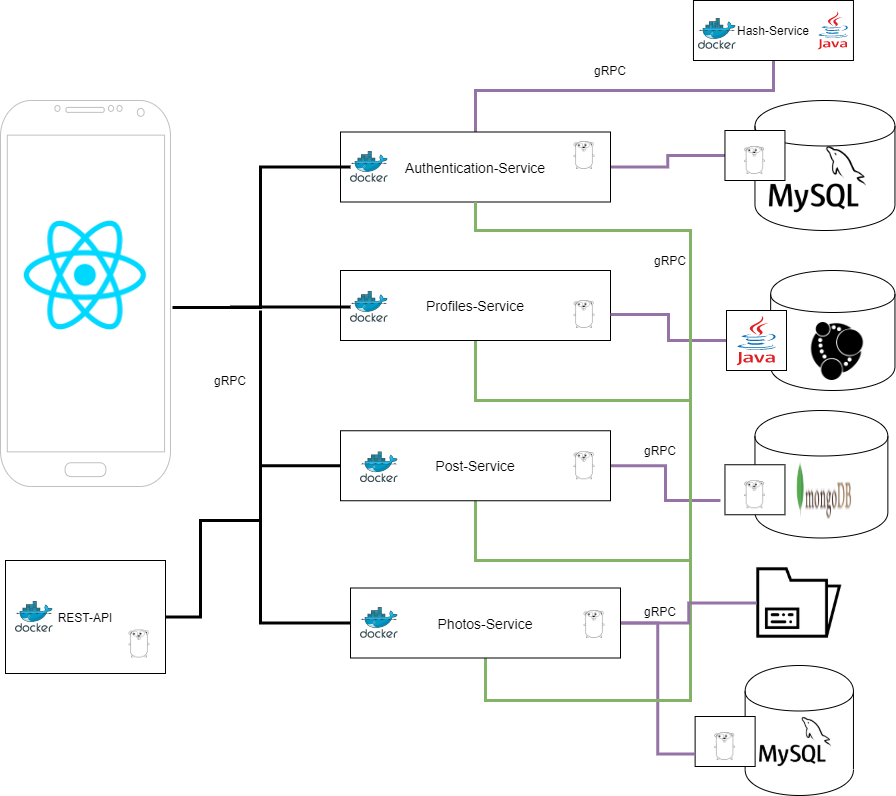
\includegraphics[width=120mm,scale=1]{img/main-uml.png}
		\caption{Application -  UML.}
		\label{application:uml}
	\end{center}
\end{figure}

\section{Objectives}
\vskip 0.1in
\indent
\indent
Doing this project, we expect to learn and prepare to afront the professional software environment, so we tried to organize our work in such a way that would imitate the real-world software development process, including the use of best practices and contemporary tools.
 The main objective of this project is to learn as much as we can to be ready to start our professional path in the software industry.
  Some of the objectives that we expect to achieve by doing this project are:
\begin{itemize}
	\item Research and learn new technologies that are utilized in the software industry.
	
	\item To improve soft skills, including teamwork, critical thinking, time management, and problem-solving.
	
	\item Apply agile techniques to develop an application based on initial requirements.
	
   	\item 	Develop a scalable microservices distributed system to manage a dynamically growing database. 
	
	\item Implement the system on the internet using the most popular cloud providers.
	Develop an application that efficiently works with images.
	
	\item Implement a reliable authentication system that securely stores passwords using hash and salt.
	
	\item To create a CRUD (create, read, update, delete) application.
	
	\item Develop a high-performance mobile application that integrates the microservices.
	
	\item Develop a REST API that integrates the microservices.
	
	\item Works in a team utilizing flourishing software development tools.
\end{itemize}


\section{Design overview}
\indent
\indent
In this project, we utilize cutting-edge technologies to develop a micro-service application.   The application is developed using relational, document base, and graph databases. We look at the benefits of each database, and we use them where we can maximize performance base on how the data is store and access on each type of database.

The System is composed of a total of 10 applications: 4 primary services, 1 hashing service, 4 database access applications, and the REST service. The services use  4 databases and 1 file storage bucket (Figure \ref{application:uml}). All services are encapsulated, perform a specific task, they communicate using gRPC, and run in a docker container.

The advantages that we want from developing the application as a distributed system are \cite{dsbook}:

\begin{itemize}
	\item Avoid expensive queries for fast performance. We use multiples databases to store the data in a simple way that makes access very fast. We avoid joins and any expensive query.
	
	\item	Scalability, each component performs a specific task; more instances of each service can be added.
	
	\item	Flexibility, each service is independent and composed of independents components as well; more components to perform a different task can be added on each service can be added, and new services can be created for a completely new task.
	
	\item Maintainability, services are easy to maintain because they are encapsulated and perform simple tasks.
	
\end{itemize}



\subsection{The Solution}
\indent
\indent
We have designed a tourism application where users create the data.  It stores data about three main types: users, cities, and places; all three have a public profile(public to register users of the application). Users create the cities and the places, and they can be created only once. Cities and places have a profile where users can post. Users can mark Cities and places as visited, so they show in their profiles and have actualization about recent posts.

In brief, it is a social media application similar to TripAdvisor. The main features of the application are 

\begin{itemize}
	 

\item Register/login/logout.
\item Create a city if a city is not yet created (add photo and description).
\item Add a place in a city (add photo and description).
\item Write a post about a city (add photo and description).
\item Visit a city (all visited cities displayed in his/her profile).
\item Visit a place (all visited places displayed in his/her profile)read .reviews/posts about a city.
\item Review all the cities that were created.
\item Review places in the city that were added.
\item Review all posts about a place.
\item Change information about himself/herself (upload photo, change. name, and description) in settings.
\item Review all the personal information in the profile (photo, geolocation, email, name, description).
\item Search a city.

\end{itemize}

\subsection{The Microservices}

The application is divided into four main microservices:
\begin{itemize}
	\item The authentication service provides secure authentication storing passwords in binary format using hash and salt.
 \item	The profiles-service store primary data of all profiles.
\item	The post-service, store, and manage posts.
\item	The photo-service, manage, and stores photo for profiles and posts. 
\end{itemize}




\subsection{Databases Design}

Each service has its database. We have research best database that fits each of the services:
\begin{itemize}
	\item The authentication service uses a relational database. When a user login a token is generated, that token can be used to authenticate each request that the user performs. A leader/slave replication has been set up to improve performance. The read from the database is distributed on multiple databases to perform the most used operation that is to authenticate requests.
	
	\item	The profiles services use a graph database. We used the graph database to create relations that avoid complicated queries.
	
	\item The post-service use a document-based database. Posts are indexed and stored in scalable documents. We can use inexpensive queries to perform CRUD operations in the posts of a city or place.
	
	\item	The photo-service store images in the file system and use a relational database to store URLs. Binary images have public access from the file system, so the image is loaded directly from the client without the need to send the image through the service, the service store URL which is sent to the user.

\end{itemize}

\subsection{Technologies introduction}
\vskip 0.1in
\indent
\indent
After some research, we decide to use Goland as the main back end programing language; some parts of the system were also writing using Java. 

We have used gRPC as the communication interface for the microservices because it provides a transparent client/ server relation. We created a go module with all gRPC interfaces that can be imported in all the components of the application.

All the services are run using docker containers, and the images are published in Docker Hub and then pulled from virtual machines to run the service. 

We have work with the 3 most popular internet services providers(Azure, google cloud, and AWS), all of them offer free student credit, and we use that. In general, the 3 services have excellent performance and outstanding support, which was used several times to learn and fix errors.

We find that one of the best for us was google cloud because they live chat and convenient SSH on the browser.  Also, the container optimized OS is outstanding to work with docker images. 


\subsection{Methodology}
\vskip 0.1in
\indent
\indent
The project has been developed in an iterative approach based on agile principles, based on the original principles we have created an adaptation to feet the demands of our project.

We define stages that are reviewed during all the project development, measure progress based on the working code, continuously meet with the team, and be ready to adapt to any change in circumstances.

The solution was created component by component, integrating them after several independent testing, we keep a working solution all the time to which we integrate more components as they are developed.


\section{Authors}
\vskip 0.1in
\indent
\indent
Authors of this dissertation are: Jose Retamal and Elena Makarenko. Introduction and Conclusion of the current paper were written in cooperation. 
Each of the rest of the chapters: Methodology,Technology Review, System Design, System Evaluation, were divided into two parts: back-end side of the application and front-end side, each part was done by Jose Retamal and Elena Makarenko respectively.

\section{Overview}
\vskip 0.1in
\indent
\indent

The structure of our dissertation is divided into chapters, each one containing different aspects of the project. A brief overview of the content of each chapter is provided below:

\subsection{Methodology (Chapter 2)}
This section outlines the methodologies that were used in order to ensure the project's success.
Mainly it describes Agile methodology, version control tool, and testing.
It also explains the criteria to chose languages, platforms, and technologies that were used.


\subsection{Technology Review (Chapter 3)}

In this section, we research and decide the best technologies to use in each component of the application. We base our research on the criteria set in the methodology.  Then we reviewed the technologies, describe it, and give an assessment.

\subsection{System Design (Chapter 4)}
This section provides a detailed explanation of the overall system architecture, thoroughly describing each component in the system. We describe how those components are linked together and how they communicate.

\subsection{System Evaluation (Chapter 5)}
We show how the system works and how the testing is performed.
It also criticizes limitations and advantages by taking a detailed look at the pros and cons of the technologies that were used.
Screenshots of the final UI can be found here as well.
We also talk about the problems encountered while developing this project and solutions to those problems. 
\subsection{Conclusion (Chapter 6)}
This section of the dissertation evaluates our project against the objective. We look at the achieved goals, set a path of progress, and analyze challenges encounter during the development of the project.


